\documentclass{article}
\usepackage[english]{babel}
\usepackage[a4paper,top=2cm,bottom=2cm,left=3cm,right=3cm,marginparwidth=1.75cm]{geometry}
% Useful packages
\usepackage{color}%\textcolor;\color
\usepackage{amsmath}
\usepackage{graphicx}
\usepackage[colorlinks=true, allcolors=black]{hyperref}
\usepackage{float}%图片包
% %create figure in latex
% \usepackage{tikz}
\usepackage[backend=bibtex]{biblatex}
%more math symbols
\usepackage{amssymb}
% %more sections
\usepackage{titlesec}
% %more sections to 5
% \newcommand{\subsubsubsection}[1]{\paragraph{#1}\mbox{}\\}% 把paragraph命令重命名为\subsubsubsection
% \setcounter{secnumdepth}{4} % 添加标号
% \setcounter{tocdepth}{4} % 添加到目录中
% \newcommand{\subsubsubsubsection}[1]{\subparagraph{#1}\mbox{}\\} % 把subparagraph命令重命名为\subsubsubsubsection
% \setcounter{secnumdepth}{5} % 添加标号
% \setcounter{tocdepth}{5} % 添加到目录中
%Information to be included in the title page:
\title{QC-Module}
\author{Xin-Peng Li}
%Start of the document
\begin{document}
\maketitle
%Generate the table of contents
\tableofcontents
\thispagestyle{empty}
\setcounter{page}{0}
\newpage
\section{DSE}
The Dyson-Schwinger equation (DSE) in the Euclidean space takes the following form
\begin{equation}
    S^{-1}\left(p\right)=Z_2\left(i\gamma\cdot p+m_{f}\left(\Lambda^2\right)\right)+\int_{q}^{\Lambda}g^2D_{\mu\nu}\left(p-q\right)\frac{\lambda^a}{2}\gamma_{\mu}S\left(q\right)\Gamma_{\nu}^{a}\left(q,p\right).
\end{equation}
The dressed-quark propagator takes the form
\begin{equation}
    S^{-1}\left(p\right)=\frac{1}{Z\left(p^2,\zeta^2\right)}\left({i\gamma\cdot p+M\left(p^2,\zeta^2\right)}\right)=i\gamma\cdot pA\left(p^2,\zeta^2\right)+B\left(p^2,\zeta^2\right).
\end{equation}
Then we apply the rainbow approximation
\begin{equation}
    \Gamma_{\nu}^{a}=\gamma_{\nu}\frac{\lambda^a}{2},
\end{equation}
and the Qin-Chang form
\begin{equation}
    g^2D_{\mu\nu}\left(k\right)=\mathcal{G}\left(k^2\right)T_{\mu\nu}\left(k\right),
    \end{equation}
where
\begin{equation}
    k^2T_{\mu\nu}\left(k\right)=k^2\delta_{\mu\nu}-k_{\mu}k_{\nu}
\end{equation}
and
\begin{equation}
    \frac{1}{Z_{2}^2}\mathcal{G}\left(k^2\right)=\frac{8\pi^2D}{\omega^4}e^{-\frac{k^2}{\omega^2}}+\frac{8\pi^2\gamma_m\mathcal{F}\left(k^2\right)}{\ln[\tau+\left(1+\frac{k^2}{\Lambda_{QCD}^2}\right)^2]}.
\end{equation}
The parameters are listed below:
\begin{equation}
    \begin{split}
        D&=1.024 GeV^2,\\
        \omega&=0.5 GeV,\\
        m_t&=0.5 GeV,\\
        \tau&=e^2-1,\\
        n_f&=4,\\
        \Lambda_{QCD}&=0.234 GeV,\\
        \gamma_m&=12/(33-2n_f).
    \end{split}
\end{equation}
The results are shown in Fig.1.
\begin{figure}[H]
    \centering
    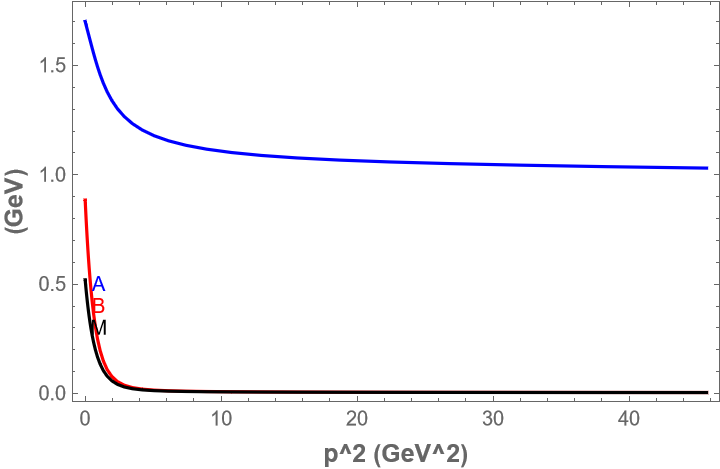
\includegraphics[width=0.8\textwidth]{Real-dse.png}
    \caption{The function A, B and the quark mass function M.}
\end{figure}
\section{BSE}
The quark-antiquark bound state amplitude can be obtained by solving a homogeneous BSE. Employing the ladder truncation becomes
\begin{equation}
    \Gamma^{f\widetilde{g}}\left(p,P\right)=-Z_2^2\int_{q}^{\Lambda}\mathcal{G}\left(k^2\right)T_{\mu\nu}\left(k\right)\frac{\lambda^a}{2}\gamma_{\mu}S^f\left(q_+\right)\Gamma^{f\widetilde{g}}\left(q;P\right)S^g\left(q_-\right)\frac{\lambda^a}{2}\gamma_{\nu}.
\end{equation}
Soving the eigenvalue equation
\begin{equation}
    \lambda\left(P^2\right)\overrightarrow{F}_X\left(P^2\right)=\mathcal{K}_X\left(P^2\right)\overrightarrow{F}_X\left(P^2\right),
\end{equation}
The solution at $\lambda\left(P^2=-M^2\right)=1$ corresponds to meson bound state.\\
The results are shown in Fig.2.
\begin{figure}[H]
    \centering
    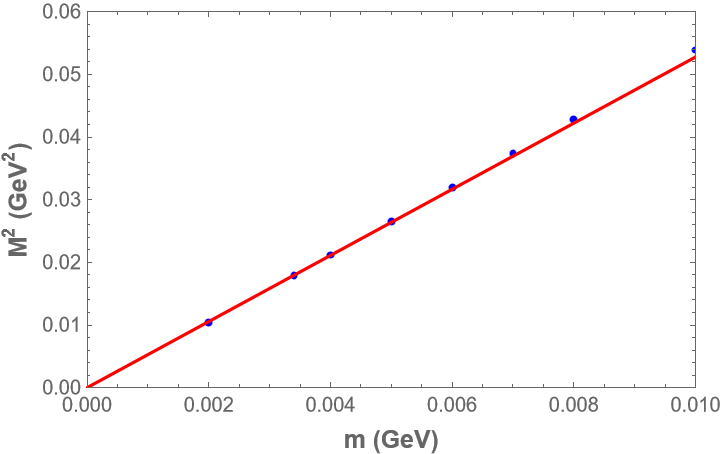
\includegraphics[width=0.8\textwidth]{pm-M^2.png}
    \caption{The blue points are directly calculated points.}
\end{figure}
This figure shows the Gell-Mann-Oakes-Renner relation.\\
I also calculate the pion decay constant $f_{\pi}$, the results are shown in the table below.
\begin{table}[H]
    \centering
    \begin{tabular}{|c|}
    \hline
    $f_{\pi}$ \\
    \hline
    0.093665 \\
    \hline
    \end{tabular}
    \caption{The pion decay constant.}
\end{table}

\end{document}